\begin{center}
	\Huge
	Kontinuitet
\end{center}


\section*{Grænseværdier og kontinuitet}
\stepcounter{section}

Vi kan bruge grænseværdibegrebet til at definere \textit{kontinuitet}. Kontinuitet for en funktion beskrives oftest løst som at vi kan tegne grafen for funktionen uden at løfte blyanten. Vi vil dog definere det lidt mere præcist ud fra grænseværdibegrebet. Igen tages der udgangspunkt i et eksempel

\begin{exa}
	Vi kan sagtens have grænseværdier, hvor der ikke indgår uendelighed. Vi betragter nu funktionen 
	$h:\mathbb{R} \to \mathbb{R}$ givet ved
	\begin{align*}
		h(x) = 
		\begin{cases}
		-x^2 + 6, \ &\textnormal{hvis } x < 2, \\
		5, &\textnormal{hvis } x = 2, \\
		3x - 4, &\textnormal{hvis } x > 2. 
		\end{cases}
	\end{align*}
	Vi kan se grafen for $h$ på Figur \ref{fig:grænse3}.
	\begin{figure}[H]
	\centering
	\begin{tikzpicture}
	\begin{axis}[
		axis lines = center, 
		xmin = -3, xmax = 5, 
		ymin = -3, ymax = 7,
		ytick = {-3,-2,...,6,7},
		xlabel = $x$, ylabel = $y$,
	]
		\addplot[color = teal, thick, domain = -3:2, samples = 100] {-x^2 + 6};
		\addplot[color = teal, thick, domain = 2:5, samples = 100] {3*x -4};
		\filldraw[color = teal] (axis cs: 2,5) circle (2pt);
		\filldraw[color = white] (axis cs: 2,2) circle (2pt);
		\draw[color = teal] (axis cs: 2,2) circle (2pt);
	\end{axis}
	\end{tikzpicture}
	\caption{Graf for funktionen $h$.}
	\label{fig:grænse3}
	\end{figure}
	For $h$ har vi grænseværdierne fra højre og venstre givet ved 
	\begin{align*}
		\lim_{x \to 2^+} h(x) = 2
	\end{align*}
	samt 
	\begin{align*}
		\lim_{x \to 2^-}h(x) = 2,
	\end{align*}
	så grænseværdien for $h$ for $x \to 2$ eksisterer og er lig $2$. Derimod har vi funktionsværdien 
	\begin{align*}
		h(2) = 5, 
	\end{align*}
	så funktionsværdien i punktet er derfor ikke lig med grænseværdien. Derfor siges $h$ ikke at være 
	kontinuert i $2$. 
\end{exa}

Kontinuitet for en funktion defineres nu som følgende. 
\begin{defn}[Kontinuitet]
	En funktion $f$ siges at være \textit{kontinuert i et punkt $x_0$}, hvis grænseværdien for $f$ eksisterer i 
	punktet $x_0$ og er lig funktionsværdien i punktet, altså at
	\begin{align*}
		\lim_{x \to x_0} f(x) = f(x_0).
	\end{align*}	 
	Hvis $f$ er kontinuert i ethvert punkt i sin definitionsmængde, så siges $f$ at være \textit{kontinuert}.
\end{defn}



\newpage

\subsection*{Opgave 1}
Grafen for funktionen $f$ kan ses på Figur \ref{fig:kont1}.

\begin{figure}[H]
	\centering
	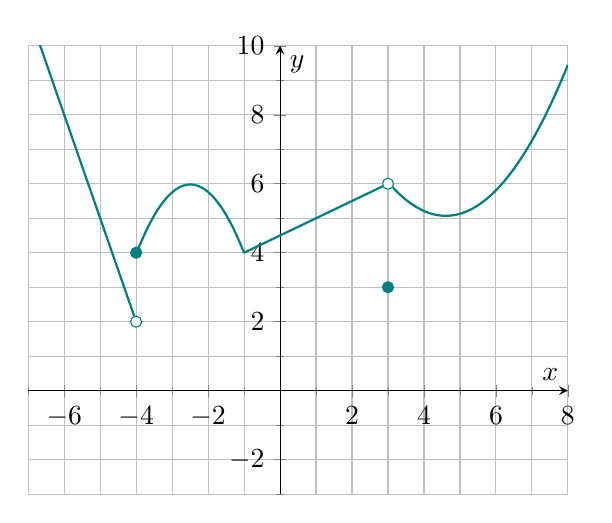
\begin{tikzpicture}
	\begin{axis}[
		axis lines = center, 
		xmin = -7, xmax = 8, 
		ymin = -3, ymax = 10,
		xlabel = $x$, ylabel = $y$,
		minor tick num = 1,
		grid = both,
	]
		\addplot[color = teal, thick, domain = -7:-4] {-3*x - 10};
		\addplot[color = teal, thick, domain = -4:-1, samples = 100] {-0.89*x^2-4.44*x+0.44};
		\addplot[color = teal, thick, domain = -1:3, samples = 100] {0.5*x + 4.5};
		\addplot[color = teal, thick, domain = 3:8, samples = 100] {0.38*x^2-3.5*x + 13.13};
		%Circle1
		\filldraw[color = white] (axis cs: -4,2) circle (2pt);
		\draw[color = teal] (axis cs: -4,2) circle (2pt);
		%Circle2
		\filldraw[color = teal] (axis cs: -4,4) circle (2pt);
		%Circle3
		\filldraw[color = white] (axis cs: 3,6) circle (2pt);
		\draw[color = teal] (axis cs: 3,6) circle (2pt);
		%Circle4
		\filldraw[color = teal] (axis cs: 3,3) circle (2pt);
	\end{axis}
	\end{tikzpicture}
	\caption{Graf for funktionen $f$.}
	\label{fig:kont1}
\end{figure}
\begin{enumerate}[label=\roman*)]
	\item Bestem tallene $f(-4)$, $f(-1)$, $f(1)$ og $f(3)$. 
	\item Bestem følgende grænseværdier
	\begin{align*}
		&1) \ \lim_{x \to -4^-}f(x) &   &2) \ \lim_{x \to -4^+}f(x) \\
		&3) \ \lim_{x \to -1^-}f(x) &   &4) \ \lim_{x \to -1^+}f(x) \\
		&5) \ \lim_{x \to 3^-}f(x) &   &6) \ \lim_{x \to 3^+}f(x) \\
	\end{align*}
	\item I hvilke af punkterne $-4$, $-1$ og $3$ eksisterer grænseværdien?
	\item I hvilke af punkterne $-4$, $-1$ og $3$ er $f$ kontinuert?
\end{enumerate}

\newpage

\subsection*{Opgave 2}
Grafen for funktionen $g$ kan ses på Figur \ref{fig:kont2}.
\begin{figure}[H]
	\centering
	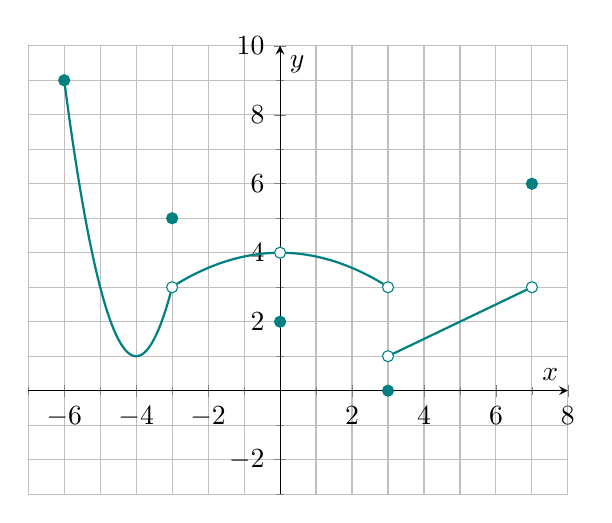
\begin{tikzpicture}
	\begin{axis}[
		axis lines = center, 
		xmin = -7, xmax = 8, 
		ymin = -3, ymax = 10,
		xlabel = $x$, ylabel = $y$,
		minor tick num = 1,
		grid = both,
	]
		\addplot[color = teal, thick, domain = -6:-3, samples = 100] {2*x^2+16*x+33};
		\addplot[color = teal, thick, domain = -3:3, samples = 100] {-0.11*x^2 + 4};
		\addplot[color = teal, thick, domain = 3:7, samples = 100] {0.5*x-0.5};
		\filldraw[color = teal] (axis cs: -6,9) circle (2pt);		
		\filldraw[color = white] (axis cs: -3,3) circle (2pt);
		\draw[color = teal] (axis cs: -3,3) circle (2pt);
		\filldraw[color = teal] (axis cs: -3,5) circle (2pt);
		\filldraw[color = white] (axis cs: 0,4) circle (2pt);
		\draw[color = teal] (axis cs: 0,4) circle (2pt);		
		\filldraw[color = teal] (axis cs: 0,2) circle (2pt);
		\filldraw[color = white] (axis cs: 3,3) circle (2pt);
		\draw[color = teal] (axis cs: 3,3) circle (2pt);		
		\filldraw[color = white] (axis cs: 3,1) circle (2pt);
		\draw[color = teal] (axis cs: 3,1) circle (2pt);
		\filldraw[color = teal] (axis cs: 3,0) circle (2pt);
		\filldraw[color = white] (axis cs: 7,3) circle (2pt);
		\draw[color = teal] (axis cs: 7,3) circle (2pt);
		\filldraw[color = teal] (axis cs: 7,6) circle (2pt);		
	\end{axis}
	\end{tikzpicture}
	\caption{Graf for funktionen $f$.}
	\label{fig:kont2}
\end{figure}
\begin{enumerate}[label=\roman*)]
	\item Bestem tallene $f(-6)$, $f(-3)$, $f(0)$, $f(3)$ og $f(7)$
	\item Bestem grænseværdierne i punkterne $-6$, $-3$, $0$, $3$ og $7$, hvis de eksisterer.
	\item Afgør, om $f$ er kontinuert i disse punkter. 
\end{enumerate}

\subsection*{Opgave 3}

Lad $f$ være givet ved
\begin{align*}
	f(x) =
	\begin{cases}
		6x - 1, &\textnormal{ hvis } x < 3,\\
		2x^2 + 4x - 8, &\textnormal{ hvis } x \geq 3. 
	\end{cases}
\end{align*}

\begin{enumerate}[label=\roman*)]
	\item Bestem $\lim\limits_{x \to 3^{-}}f(x).$
	\item Bestem $\lim\limits_{x \to 3^{+}}f(x).$
	\item Bestem $f(3)$.
	\item Afgør, om $f$ er kontinuert i 3.
\end{enumerate}

\subsection*{Opgave 4}
\begin{enumerate}[label=\roman*)]
	\item Afgør, om funktionen $g$ givet ved
	\begin{align*}
		g(x) = 
		\begin{cases}
			x^3 + 7, &\textnormal{ hvis } x < -2,\\
			-3x^2- 5x + 1, &\textnormal{ hvis } x \geq -2. 
		\end{cases}
	\end{align*}
	er kontinuert i punktet $-2$.
	\item Afgør, om funktionen $h$ givet ved
	\begin{align*}
		h(x) =		
		\begin{cases}
			\cos(x) - 4, &\textnormal{ hvis } x < 0,\\
			\sin(x) - 3, &\textnormal{ hvis } 0\leq x < 1, \\
			2, &\textnormal{ hvis } x = 1, \\
			-3x^2 + 1 , &\textnormal{ hvis } x > 1, \\ 
		\end{cases}
	\end{align*}
	har nogle punkter, hvor grænseværdien ikke eksisterer. Overvej derefter, om $h$ har nogle diskontinuiteter.
\end{enumerate}


\subsection*{Opgave 5}
Har vi et udtryk $\sqrt{x} + a$, så kalder vi udtrykket $\sqrt{x} - a$ for det konjugerede udtryk. Dette kan ofte bruges til at bestemme grænseværdier med 0/0-udtryk. 
\begin{enumerate}[label=\roman*)]
	\item Vi ønsker at bestemme grænseværdien
	\begin{align*}
		\lim_{x \to 4} \frac{\sqrt{x}-2}{x-4}.
	\end{align*}
	Forlæng først brøken med det konjugerede udtryk $\sqrt{x}+2$. 
	\item Gang udtrykket i tælleren sammen, men lad parenteserne i nævneren stå.
	\item Forkort udtrykket og evaluér grænseværdien
\end{enumerate}

Bestem følgende grænseværdier, der giver 0/0-udtryk ved at forlænge med det konjugerede udtryk. 

\begin{align*}
	&1) \ \lim_{x \to 9} \frac{\sqrt{x}-3}{x-9}    & &2) \ \lim_{x\to 3}\frac{\sqrt{x+1} - 2}{x-3}  \\
	&3) \ \lim_{x \to 0} \frac{\sqrt{x + 1} - 1}{x}  & &4) \ \lim_{x \to 4} \frac{\sqrt{x^2 -12}-2}{x-4}  \\
\end{align*}

\subsection*{Opgave 6}
En mere stringent definition af grænseværdier lyder som følgende.
\begin{defn}[Grænseværdi]
	En funktion $f: \mathbb{R} \to \mathbb{R}$ siges at have grænseværdien $L$ i et punkt
	$x_0$, hvis der for ethvert tal $\varepsilon > 0$ findes et tal $\delta > 0$ så
	 hvis det for $x \neq x_0$ så $0 < |x - x_0| < \delta$ medfører, at $0 < |f(x) - L| < \varepsilon$.
\end{defn}
Overvej, hvad $\delta$ skal være, hvis $\varepsilon = 1$ i opgaverne fra Opgave 1. 
